\section{Motivation}
In geschlossenen physikalischen Systemen gilt die Energierhaltung. Doch was genau das anschulich bedeutet
soll dieser Versuch unter anderem Vermitteln. In diesem Versuch ist das Ziel die Einwirkung von dem Trägheitsmoment
auf das Beschleunigungsverhalten auf einer schiefen Ebene zu beobachten und daraus auf die Energierhaltung zu schließen.
ZU beobachten ist das Phänomen im Alltag, beispielswiese beim Fahrradfahren. Dort wäre es interessant zu wissen, welche Geometrie der Felgen optimal ist,
um die geringsten Geschwindigkeitseinbußen beim bergabfahren zu haben.


\section{Messverfahren}
Zuerst wurden Ebene und Körper vermessen um einen Überblick über die Größen zu gewinnen.
Die Messung beinhaltete drei Körper, einen Vollzylinder aus Aluminium, einen Hohlzylinder aus Messing und einen Verbunzylinder mit Aluminiumhülle und Messingkern.
Diese wurden die schiefe Ebene herabgerollt. Dabei wurde die Zeiten mittls Lichtschranken in quadratischen Längenabständen gestoppt.
Daraus soll die Beschleunigung bestimmt werden. \\
Im zweiten Teil werden zwei der vier Lichtschranken an die flache Ebene, welche unten an die schiefe Ebene anschloss, gesetzt.
Mithilfe dieses Aufbasu kann die Endgeschwindgkeit und daraus die kinetische Energie bestimmt werden.\\
Zur Zeitmessung waren vier Lichtschranken vorhanden, welche über den Hebel, welcher die Körper rollen ließ, automatisch aktiviert.
Beim durchlaufen der Lichtschranken werden die Zeiten elektrisch gestoppt.

\section{Aufbau}

\begin{figure}[h!]
    \centering
    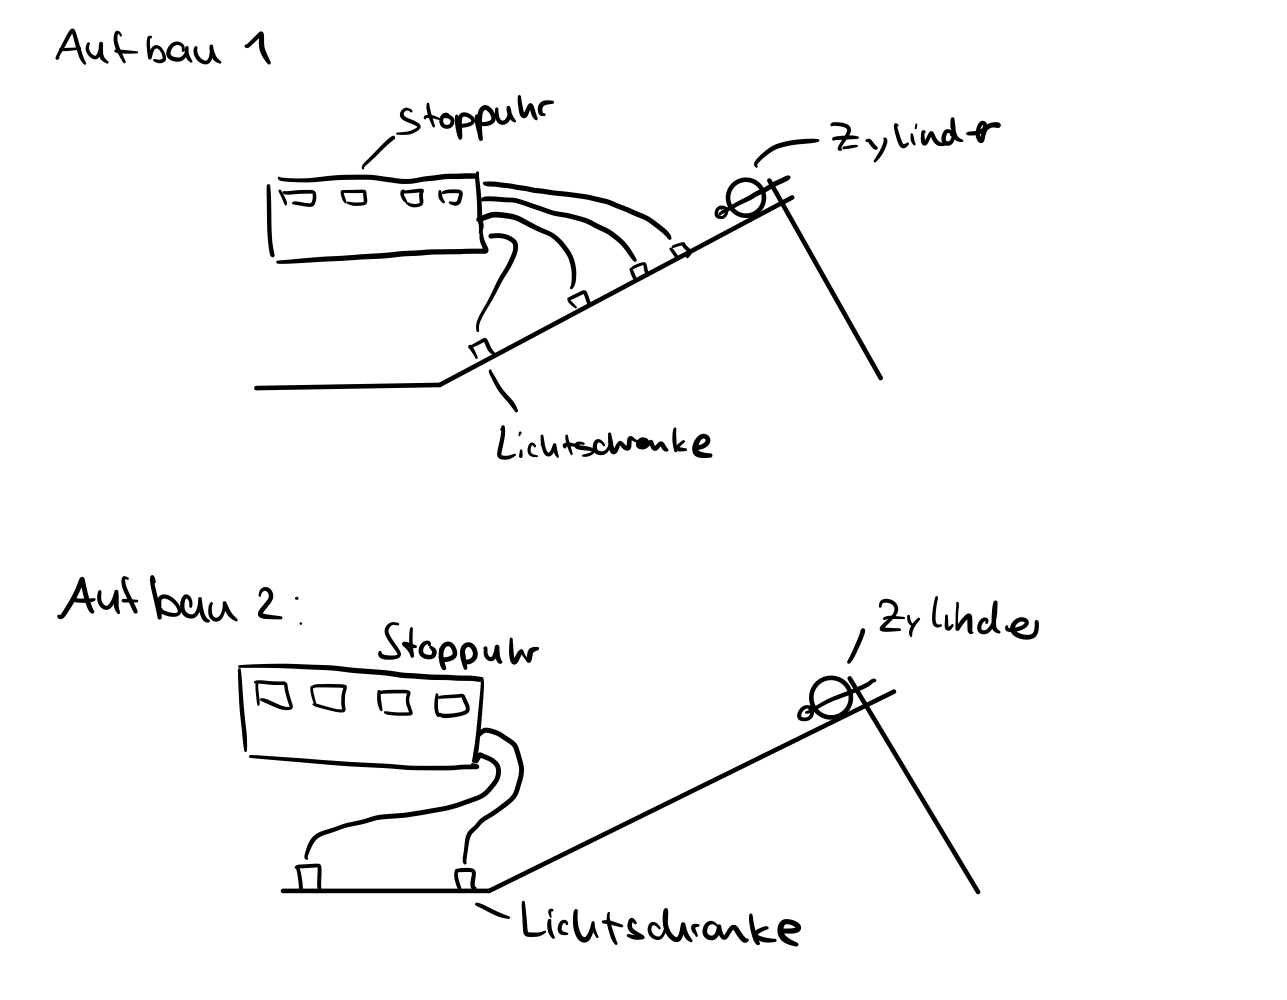
\includegraphics[width = .7\textwidth]{Aufbau15.jpeg}
\end{figure}
\newpage

\section{Grundlagen aus der Physik}

\subsection{Schiefe Ebene}
Auf der schiefen Ebene wirken mehrere Kräfte gleichzeitig. Zuerst wurkt der parallel zur Ebene verlaufene Anteil der Gravitationskraft die Hangabtriebskraft $F_{HA}$.
Der senkreechte Anteil wird genau durch die Normalkraft aufgehoben.
Zusätzlich gibt es in der realen schiefen Ebene die Reibungskraft $F_R$. Diese erzeugt ein Drehmoment auf den Körper.
DAbei gilt fürr das Drehmoment mit $J$ als Trägheitsmoment und $r$ als Radius des Körpers:
\begin{equation}
    M = F_R \cdot r = J\dot \omega
\end{equation}
Dabei beschreibt $\omega$ die Winkelgeschwindigkeit. Teilt man beide Seiten durch den Radius erhält man einen Ausdruck für die Reibungskraft.
Da diese entgegen der Hangabtriebskraft wirkt ergibt sich ein negatives Vorzeichen:
\begin{equation}
    F_{ges} = F_{HA}-F_R
\end{equation}
Setzt man nun die Ausdrücke ein erhält man einen Ausdruck für die Beschleunigung $a$, dabei ist $m$ die Masse des Körpers und $\alpha$ der Winkel der Ebene.

\begin{align}
    ma & = mg\sin(\alpha)- J\frac{a}{r^2} \\
    \Rightarrow a &=\frac{mg \sin(\alpha)}{m + \frac{J}{r^2}} \\
    \Rightarrow a  &=\frac{mg h}{l (m + \frac{J}{r^2})} \label{eq:a}
\end{align}
Der Winkel ergibt sich aus der Höhe der Ebene $h$ un der Lände der Ebene (Hypotenuse) $l$.

\subsection{Trägheitsmomente}

Für das Trägheitsmoment eines Körpers gilt allgemein:
\begin{equation}
    \int_V \rho(r)\cdot r_{\bot}\  dV
\end{equation}
Dabei ist $r_\bot$ der Abstand der sekrechten zur Rotationsrichtung, $\rho$ die Dichte und $V$ das Volumen.
Aus dieser Gleichung lässt sich das Trägheitsmoment folgender rotationssymmetrischer Körper mit Masse $m$ und Radius $r$ bestimmen:
\textbf{Vollzylinder}:

\begin{equation}
    J_V = \frac{1}{2} mr^2
    \label{eq:JVoll}
\end{equation}

\textbf{Hohlzylinder}:

\begin{equation}
    J_H = \frac{1}{2}m (r_2^2 + r_1^2)
    \label{eq:JHohl}
\end{equation}

Dabei beschreibt $r_2$ den Außenradius und $r_1$ den Innenradius.

\subsection{Kinetische Energie}

Körper mit Masse $m$ und Geschwindigkeit $v$ oder Trägheitsmoment $J$ und Rotationsgeschwindigkeit $\omega$ besitzen eine sogenannte kineetische Energie.
Diese setzt sich aus der Translations- und Rotationsenergie zusammen.
Die Translationsenergie ist die Energie die eine Körper bei translatorisch Bewegung besitzt. Diese lässt sich berechnen durch:
\begin{equation}
    E_{trans} = \frac{1}{2}m v^2 = \frac{1}{2}m\left(\frac{s}{\Delta t}\right)^2
    \label{eq:ETrans}
\end{equation}

Mit $s$ als überschrittene Fläche in $\Delta t$ Zeit.

Rotiert ein Körper um sich selbst ergibt sich eine Drehbewegung um den Schwerpunkt, die Energie die ein Körper dabei besitzt wird durch folgende Gleichung beschreiebem.

\begin{equation}
    E_{rot} = \frac{1}{2}J \omega^2 = \frac{1}{2}J\left(\frac{s}{r \Delta t }\right)^2
    \label{eq:ERot}
\end{equation}

Die Summe der Beiden nennt man dann kinetische Energie.\\
Bewegt sich ein Körper im Schwerefeld der Erde so besitzt dieser eine potentielle Energie.
Diese beschreibt die in einem Körper vorhandene Energie in referenz zu einem anderen Punkt. Die Höhendifferenz beschreibt hier $h$.

\begin{equation}
    E_{pot} = mgh
    \label{eq:pot}
\end{equation}

In dem Protkoll wird as Erdbeschleinigung $g=\SI{9,81}{\frac{\meter}{\second^2}}$
